% !Mode:: "TeX:DE:UTF-8:Main"

\documentclass[aspectration=169]{beamer}
\usepackage{tikz}
\usetikzlibrary{tikzlings,ducks}
\usepackage[x11names,svgnames]{xcolor}
\usepackage{eso-pic}
\ExplSyntaxOn
\AddToHook{shipout/background}%
 {\put(0,-\paperheight){%
\includegraphics[page=\int_eval:n{\int_mod:nn{\value{page}}{10}+1}]{starsky}}} 
\ExplSyntaxOff
\setbeamertemplate{background canvas}{}
\setbeamertemplate{navigation symbols}{}

\begin{document}

\newcommand\rscale{1.2} 
\newcommand\scalefactor{3380}
\foreach \i in {100,105,...,3880}{ 
\begin{frame}
\begin{tikzpicture}
\path[use as bounding box](-0.5\textwidth,-0.5\textheight)rectangle(0.5\textwidth,0.49\textheight);
\path  (0,0)  -- (\i:\fpeval{(\rscale*\i/2000)^2}) pic[scale=\fpeval{\i/\scalefactor}] {rhino}; 
\ifnum\i >300 
 \path  (0,0)  -- (\i-200:\fpeval{(\rscale*(\i-200)/2000)^2}) pic[scale=\fpeval{(\i-200)/\scalefactor}] {owl}; 
\fi
\ifnum\i >500 
 \path  (0,0)  -- (\i-400:\fpeval{(\rscale*(\i-400)/2000)^2}) pic[scale=\fpeval{(\i-400)/\scalefactor}] {mouse}; 
\fi 
\ifnum\i >700 
 \path  (0,0)  -- (\i-600:\fpeval{(\rscale*(\i-600)/2000)^2}) pic[scale=\fpeval{(\i-600)/\scalefactor}] {bear}; 
\fi 
\ifnum\i >900 
 \path  (0,0)  -- (\i-800:\fpeval{(\rscale*(\i-800)/2000)^2}) pic[scale=\fpeval{(\i-800)/\scalefactor}] {snowman}; 
\fi 
\ifnum\i >1100 
 \path  (0,0)  -- (\i-1000:\fpeval{(\rscale*(\i-1000)/2000)^2}) pic[scale=\fpeval{(\i-1000)/\scalefactor}] {cat}; 
\fi 
\ifnum\i >1300 
 \path  (0,0)  -- (\i-1200:\fpeval{(\rscale*(\i-1200)/2000)^2}) pic[scale=\fpeval{(\i-1200)/\scalefactor}] {pig}; 
\fi 
\ifnum\i >1500 
 \path  (0,0)  -- (\i-1400:\fpeval{(\rscale*(\i-1400)/2000)^2}) pic[scale=\fpeval{(\i-1400)/\scalefactor}] {coati}; 
\fi 
\ifnum\i >1700 
 \path  (0,0)  -- (\i-1600:\fpeval{(\rscale*(\i-1600)/2000)^2}) pic[scale=\fpeval{(\i-1600)/\scalefactor}] {marmot}; 
\fi 
\ifnum\i >1900 
 \path  (0,0)  -- (\i-1800:\fpeval{(\rscale*(\i-1800)/2000)^2}) pic[scale=\fpeval{(\i-1800)/\scalefactor}] {panda}; 
\fi 
\ifnum\i >2100 
 \path  (0,0)  -- (\i-2000:\fpeval{(\rscale*(\i-2000)/2000)^2}) pic[scale=\fpeval{(\i-2000)/\scalefactor}] {penguin}; 
\fi 

\ifnum\i >2300 
 \path  (0,0)  -- (\i-2200:\fpeval{(\rscale*(\i-2200)/2000)^2}) 
 pic[scale=\fpeval{(\i-2200)/\scalefactor}] {bee}; 
\fi 

\ifnum\i >2500 
 \path  (0,0)  -- (\i-2400:\fpeval{(\rscale*(\i-2400)/2000)^2}) 
 pic[scale=\fpeval{(\i-2400)/\scalefactor}] {hippo}; 
\fi 

\ifnum\i >2700 
 \path  (0,0)  -- (\i-2600:\fpeval{(\rscale*(\i-2600)/2000)^2}) pic[
 duck/santa=red!80!black, duck/jacket=red!80!gray, 
 duck/tshirt=white,duck/beard=white!80!brown,
 duck/body=LightGoldenrod2!70!RosyBrown1,
 scale=\fpeval{1.5*(\i-2600)/\scalefactor}] {duck}; 
\fi 
 
\end{tikzpicture}
\end{frame}
}

\end{document}
